% This assumes your files are encoded as UTF8
\pdfoutput=1

\documentclass[11pt]{article}

% Standard package includes
\usepackage{times}
\usepackage{latexsym}
\usepackage[utf8]{inputenc}
\usepackage[T1]{fontenc}
\usepackage{microtype}
\usepackage{float} % Add this line to the preamble
\usepackage{inconsolata}
\usepackage{graphicx} % Required for inserting images
% Adjust margins
\usepackage[papera4,margin=1in]{geometry}
\title{Fallback Dataset  -  Homework 1b }
\author{Shahkar - Matricola 2047305 }

\begin{document}
\begin{center}
    \huge{Fallback Dataset  -  Homework 1b }\\ [10pt]
    \large{Shahkar - Matricola 2047305}
\end{center}
%\maketitle

\section{Introduction:}
The task that I am working on is like a sentiment analysis given a certain sentence. I must design a model to predict the sentiment of that sentence i.e. neutral or hateful. 
\section{Dataset Description: }
The dataset that I am working on is called the fallback dataset, which consist of one training set and two test sets. Each sample has a sentence in Italian with choices ["neutrale", "odio"] followed by its correct label i.e. 0 or 1
\section{Model Architectures: } 
I implemented two models, one for baseline and the other extra for improving accuracy. The first one consists of a simple LSTM model which consist of embedding layers, a couple of LSTM layers, and a linear layer in the end. 

The second model is the LSTM-CNN Hybrid model, CNNs are excellent at capturing local patterns and features in data, while LSTMs are proficient in understanding temporal dependencies. Combining them allows for hierarchical feature extraction, where CNNs can extract low-level features, and LSTMs can learn higher-level temporal patterns from these features. CNNs are also prone to overfitting when trained on limited data, especially for tasks with small datasets. This model consists of an embedding layer followed by three 1D convolutional layers, simple LSTM layers, and then in the end linear layer for prediction.
\section{Design Choices: } 
I chose the Adam optimizer which works best in most of the LSTM models with a learning rate of 0.0001 which was found suitable after a grid search. Also, by trail and run I chose a dropout of 0.4 in my model. For a batch size of 128, I ran my model for like 30 epochs which was way more given a small training dataset.
\section{Baseline Model: } 
In baseline model which consist of a simple LSTM layer followed by a linear layer. First trained my model without any validation set the accuracy was about 48 -53 \% on both test sets, I also used early stopping just in case if the model overfit the training stop after 20 epochs because there was no improvement in loss of validation set. but it seems like the dataset is too small to acquire a decent accuracy.
\section{Results: } 
To compare the result which can also be seen in Figure 1 and Figure 2 mentioned in the appendix, a non-baseline model which is the CNN-LSTM hybrid model works slightly better than the baseline model with accuracy ranging up to 58.4\% for test set 1 and 51.9 \% for test set 2. Which can be considered a good model given such a small amount of data.

\section{Instruction to run a code: }
All code was written locally with the assumption of that the training and test JSON files are in the same folder as the notebook. So just make sure to check that. Also, it should be noted that the model may give slightly different accuracy and loss values due to the random split of the training set.

\section{Appendix:}
 Baseline model:
\begin{figure}[H] % Use [H] specifier instead of [htbp]
  \centering
  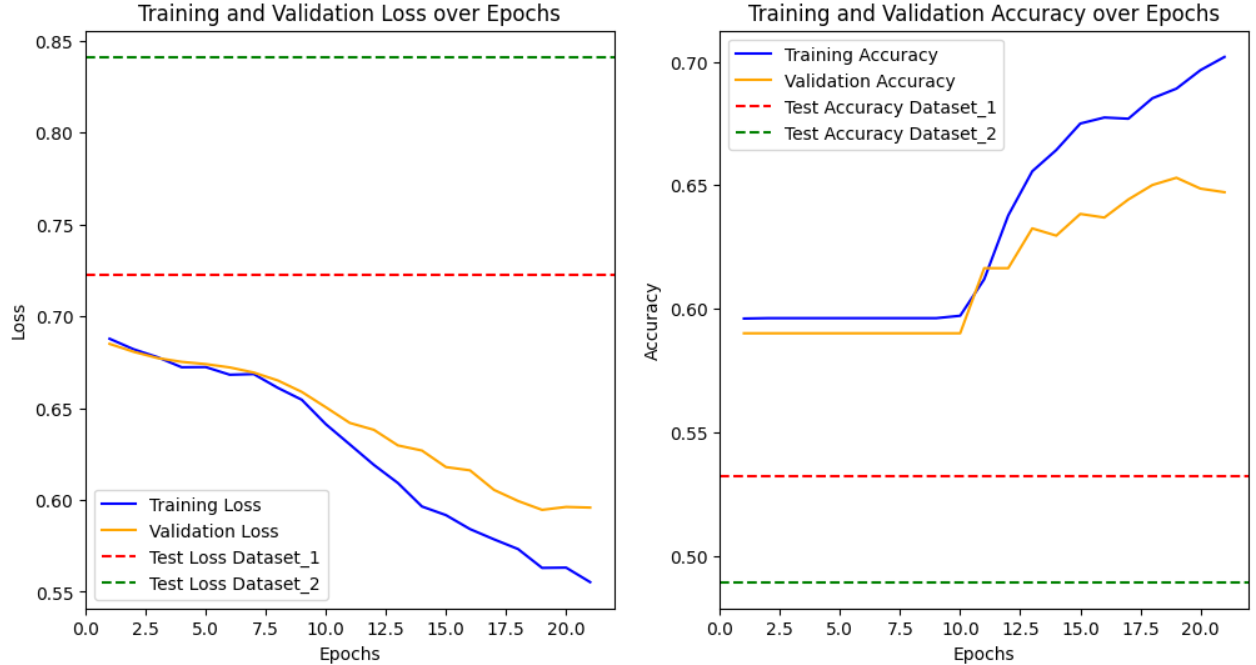
\includegraphics[width=0.5\textwidth]{baseline.png}
  \caption{Baseline model.}
  \label{fig:baseline}
\end{figure}

Extra-non baseline model:
\begin{figure}[H]
  \centering
  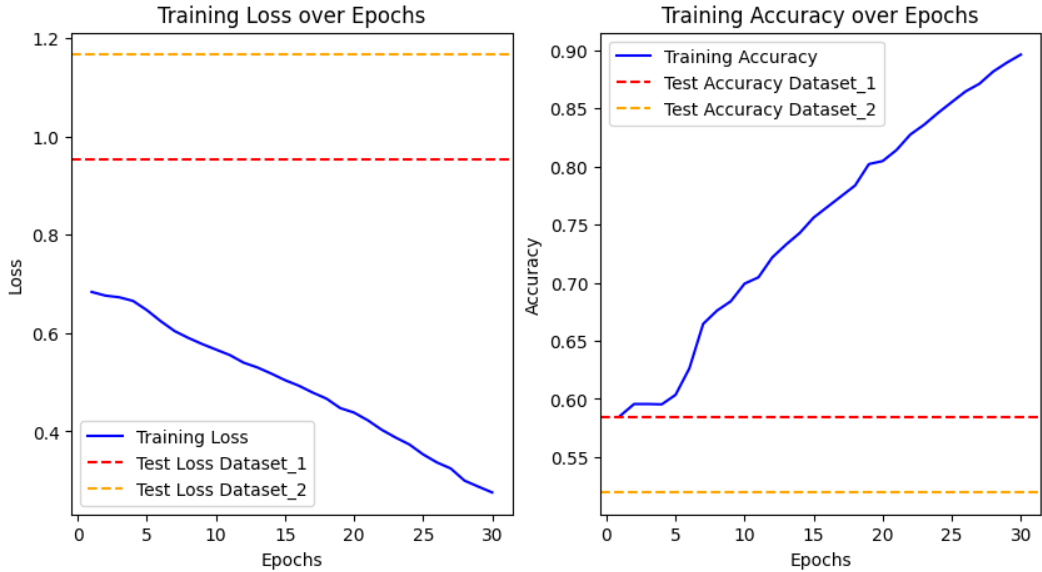
\includegraphics[width=0.5\textwidth]{Extra-Baseline.png}
  \caption{Extra-non baseline model.}
  \label{fig:extra}
\end{figure}

\end{document}
